% !TEX program = pdflatex --shell-escape

\documentclass[11pt]{article}
\usepackage[round,sort&compress,semicolon]{natbib}
\usepackage{times}
\usepackage[T1]{fontenc}
\usepackage[utf8]{inputenc}
\usepackage[pdftex]{graphicx}\usepackage[letterpaper, left=1.0in, right=1.0in, top=1.0in, bottom=1.0in]{geometry}
\usepackage{ragged2e}
\usepackage{url}
\usepackage{setspace}
\usepackage{lineno}
\usepackage{multirow}
\usepackage{pdflscape}
\usepackage[backref=page]{hyperref}
\usepackage{rotating}
\usepackage{booktabs}
\usepackage[hypcap, labelsep=period, labelfont=bf]{caption}
\usepackage{array}
\usepackage{color}
\usepackage{soul}
\usepackage{mathtools}
\usepackage{pdflscape}

\usepackage{amsmath}
\usepackage{amsfonts}       % blackboard math symbols
\usepackage{nicefrac}       % compact symbols for 1/2, etc.
\usepackage{microtype}      % microtypography
\usepackage{doi}


\usepackage[usenames,dvipsnames,svgnames,table]{xcolor}
\urlstyle{same}
\setlength{\RaggedRightParindent}{\parindent}
\linenumbers
\linespread{1.1}

% restart counting in the supplement
\newcommand{\beginsupplement}{%
	\setcounter{table}{0}
	\setcounter{figure}{0}
	% \setcounter{section}{0}
	% \setcounter{subsection}{0}	
	\renewcommand{\thetable}{S\arabic{table}}%
	\renewcommand{\thefigure}{S\arabic{figure}}%
	% \renewcommand{\thesection}{S\arabic{section}}%
	% \renewcommand{\thesubsection}{S\arabic{section}.\arabic{subsection}}%          
}

%%% Add PDF metadata to help others organize their library
%%% Once the PDF is generated, you can check the metadata with
%%% $ pdfinfo template.pdf
\hypersetup{
     colorlinks   = true,
     citecolor    = Indigo,
     linkcolor    = DarkCyan,
}

\begin{document}

\begin{center}
	{\bf \Large
Phylogenomic Evidence for Taxonomic Reevaluation in North American \textit{Delphinium} and the Dominance of Geographic Patterns}
	}\\[0.5cm]

Jared B. Meek$^{1,*}$, Daniel Cook$^2$, B. Shaun Bushman$^3$, Deren A.R. Eaton$^{1,*}$\\[0.5cm]

1. Department of Ecology, Evolution, and Environmental Biology, Columbia University, 1200 Amsterdam Ave, New York, NY, 10027, USA;\\
2. USDA-ARS Poisonous Plant Research Laboratory, 1150 E 1400 N Logan, UT, 84341, USA;\\ 3. Forage \& Range Research Lab, Utah State University, Logan, UT 84322, USA;\\ 
* Corresponding Authors: jared.meek@columbia.edu; de2356@columbia.edu
% daniel.cook@usda.gov\\
% shaun.bushman@usda.gov\\

\end{center}

Keywords: ...

\RaggedRight

\section*{Abstract}
% Western North America contains unresolved plant clades that we need to understand better
North America is a topographically and ecologically complex region that has fostered the 
diversification of many endemic plant lineages. Its unique flora includes many rare and
specialized taxa narrowly distributed along climatic gradients, which now face mounting
threats from shifting climate and precipitation patterns, increased wildfire frequency, and habitat loss
\citep{kannenberg_rapid_2021,overpeck_climate_2020}.
% 
Although the region is among the most thoroughly studied botanical areas in the world
\citep{hickman1993jepson}, persistent taxonomic uncertainties hinder our ability to
accurately quantify biodiversity and track its decline. 
These knowledge gaps limit our ability to detect local extinctions [CITE], 
estimate species range shifts [CITE], and scale ecological predictions across spatial hierarchies. 


The delimitation of species and their phylogenetic relationships remain poorly
understood even within some of the most enigmatic plant lineages of this region, 
such as larkspurs \citep{jabbour_phylogeny_2012, xiang_recircumscription_2017} 
% louseworts \citep{yu_towards_2015}, 
and paintbrushes \citep{tank_phylogenetic_2009,jacobs_quantifying_2019}.
% 
Such species-rich lineages often present taxonomic challenges owing to their 
rapid diversification and high frequency of hybridization.
% 
This is especially challenging for morphological systematics, where lineages
may be under- or over-split due to differences in rates of morphological evolution.
% 
Such patterns are likely to be exacerbated in mountainous regions, where
parallel adaptations to similar environmental gradients can cause cryptic variation,
as in the case of \emph{Viburnum} in neotropical
cloud forests \citep{donoghue_replicated_2022}. 
% 
When selection maintains distinct morphologies across environmental
gradients, as in the case of desert \emph{Encelia} 
\citep{divittorio_natural_2020}, rare hybrid populations may exhibit
distinct phenotypes that can lead to inflated species descriptions.
% 
Systematic revisions that incorporate phylogenomic evidence can better
assess the distinctiveness of taxa by combining information from molecular
phylogenies, morphology, geography, and hybrid admixture [CITE].
% 
This work contributes not only to improving plant taxonomy, but also to
our ability to quantify and preserve biodiversity; identify historical 
corridors of migration and dispersal; and investigate plant adaptations
to extreme conditions \citep{anstett_2021, gross_unforeseen_2024, melton_draft_2021}. 


A prime example of these dynamics is the North American clade of \emph{Delphinium} 
sect. \emph{Diedropetala} (Ranunculaceae), which has experienced a rapid radiation 
into approximtely 60 species since its arrival to western North America an 
estimated three million years ago \citep{jabbour_phylogeny_2012}.
% 
Species of this clade are perennial herbaceous plants characterized by large 
showy flowers that are typically blue and purple, and less commonly red, yellow, 
or white. 
% 
Many species are widespread and abundant in montane, grassland, and desert habitats,
while others exist as narrow endemics that have specialized adaptations to harsh 
alpine environments \citep{warnock_taxonomic_1995}. 
% 
Multiple species are currently endangered in North America. 
They are economically important as ornamentals, but are also intensely studied for 
their toxicity to livestock \citep{cook_2009, cook_two_2017, gardner_taxonomic_2002, pfister_grazing_2014}.
% Cook et al., 2009, 2017; Gardner et al., 2002; Pfister et al., 2014). 
Their rapid diversification in North America has been attributed to dispersal and 
isolation in the various mountain ranges of the western Cordillera, especially the
Cascades, Sierra Nevada, and Rocky Mountains \citep{Warnock_1997}.
% 
Despite multiple taxonomic and phylogenetic research efforts focused on this clade,
there is no fully resolved phylogeny of \emph{Delphinium} sect. \emph{Diedropetala},
and little is known about its biogeographic history across western North America.


The genus \emph{Delphinium} is often considered taxonomically difficult due to a 
limited number of 
%distinguishable 
distinguishing
morphological characters. Two comprehensive 
taxonomic treatments for North American \emph{Delphinium} have been published over 
the last century \citep{benson_synopsis_1946,ewan_1945, warnock_1997}, %(Ewan, 1945; Warnock, 1997),
which recognize between 60-80 species, but disagree over their exact number, 
nomenclature, and distribution. 
% 
In the first published circumscription of the clade, Ewan combined extensive 
fieldwork and study of herbarium specimens to distinguish 79 species grouped 
into 13 “series” based on seed morphology, leaf architecture and pubescence, 
corolla color, and other anatomical features. 
% 
Fifty years later, Warnock’s treatment [CITE] reduced the number of species 
from 79 to 61, comprising two sections: \emph{Elatopsis}, represented by a garden 
cultivar (\emph{Delphinium elatum}) introduced from Europe, and 
\emph{Diedropetala}, which is composed of nine subsections.
%
These subsections are largely delineated by root structure and size, 
sepal color and length, seed morphology, and fruit position.
% 
This treatment is included in the current Flora of North America 
\citep{...} (but compare with regional treatments;
\cite{ackerfield_flora_2022,chambers_comments_2018,holmgren_2012,koontz_2012}.
)
% Ackerfield, 2022; Chambers, 2018; Holmgren et al., 2012; Koontz & Warnock, 2012).


In addition to these treatments, two molecular phylogenetic studies have used
Sanger sequencing markers to examine relationships within section \emph{Diedropetala}.
% 
A study by \citet{koontz_using_2004} sampled sixty-two species of 
North American \emph{Delphinium} but found that few relationships can
be resolved using a small number of molecular markers. 
% Referencing both Ewan and Warnock’s treatments, \citet{koontz_using_2004}
% sampled sixty-two \emph{Delphinium} species from North America. 
% Their phylogenetic results showed clearly that the rapid radiation in this
% clade cannot be resolved without greater genomic sampling. 
% 
A deeper-scale phylogenetic analysis of \emph{Delphinium} conducted
by \cite{jabbour_phylogeny_2012} sampled a third of the North American species,
but included many other species from its global distribution.
Their results support \emph{Diedropetala} as a monophyletic clade that diverged
from east Asia approximately 3 Mya. 
% 
Although their study recovered high support across the genus-level 
backbone of \emph{Delphinium}, it lacked the sampling and power to 
resolve relationships within section \emph{Diedropetala}.
% 
No study has yet brought genome-scale data to bear on phylogenetic 
relationships within \emph{Delphinium}.
% , and consequently, many relationships
% among species and larger clades remains unresolved. 
%recent and rapid radiations. With less than half of the species in North America sampled, and poor resolution within this clade, the relationships among North American Delphinium species and subsections remains largely unresolved. 


% A paragraph about hybridization and the power of genomic data to resolve
Multi-locus phylogenomic analyses offer an advantage not only for inferring
species tree relationships from discordanct (conflicting) phylogenetic signals, 
but additionally for the potential to test for evidence of hybrid introgression
[CITE].
% 
Hybridization is likely to have played a significant role throughout the 
diversification of \emph{Delphinium}. 
Many putative hybrids have been described based on morphological descriptions 
\citep{ewan_1945, warnock_1997},
but the extent to which they contribute to introgressive gene 
flow between species remains unknown.
% few have been confirmed using reproductive experiments or genomic 
% sequencing, 
% 
% EXPAND THIS SECTION A BIT>
% 
% Phylogenomic approaches that utilize thousands of loci have the power to distinguish hybrid introgression from neutral sources of discordance, such as incomplete lineage sorting, or a lack of phylogenetic information. 
In this study, we generated a new reduced-representation genomic dataset to 
investigate phylogeny and introgression across the \emph{Delphinium} sect. 
\emph{Diedropetala} clade. 
% 
We present a new and highly revised phylogenetic hypothesis for relationships
among species representing all previously described subsections in this clade 
% ({\bf Fig. 1}), 
and discuss our confidence in this result with regard to our 
extensive sampling of populations within species, tests for hybrid 
introgression, and the biogeographic concordance of our results.


%%%%%%%%%%%%%%%%%%%%%%%%%%%%%%%%%%%%%%%%%%%%%%%%%%%%%%%%%%%%%%%%%%%%%%%%%%%%%%%%%%%%%%%%%%%
%%%%%%%%%%%%%%%%%%%%%%%%%%%%%%%%%%%%%%%%%%%%%%%%%%%%%%%%%%%%%%%%%%%%%%%%%%%%%%%%%%%%%%%%%%%
%%%%%%%%%%%%%%%%%%%%%%%%%%%%%%%%%%%%%%%%%%%%%%%%%%%%%%%%%%%%%%%%%%%%%%%%%%%%%%%%%%%%%%%%%%%
%%%%%%%%%%%%%%%%%%%%%%%%%%%%%%%%%%%%%%%%%%%%%%%%%%%%%%%%%%%%%%%%%%%%%%%%%%%%%%%%%%%%%%%%%%%
\section{Materials and Methods}

\subsection{Taxon sampling}
We collected voucher specimens and silica-preserved leaf samples during field expeditions
between 2019-2022. Additional samples were provided by the USDA Poisonous Plant Research
Lab as part of a long-term research program concerning toxicity in \emph{Delphinium}, where
tissues were stored freeze-dried.
% 
This dataset includes 189 individuals, with replicate samples of 34 \emph{Delphinium} 
species collected from multiple geographically disjunct populations. Our sampling includes
at least one species as a representative of each subsection in Warnock’s \emph{Delphinium}
treatment in the Flora of North America (FNA). 
We included samples from two \emph{Aconitum} species as outgroups.
All collections have associated geographic coordinates (Table S1) and voucher 
specimens available at the USDA Poisonous Plant Research Lab Herbarium (PPRL)
in Logan, UT.

\subsection{DNA sequencing and bioinformatics}
Genomic DNA was extracted from lyophilized leaf tissue using the Quick DNA
extraction kit (Zymo Research), adapted to a 96-well format. 
DNA quantity and quality were assessed using a spectrophotometer, TapeStation 
(Agilent), and gel electrophoresis, and genomic DNA was standardized to 20 ng/ul. 
% 
Genomic double-digest restriction-site associated DNA \citep[ddRAD-seq;][]{peterson_double_2012}
libraries were prepared at the USDA Forage \& Range Research Lab at 
Utah State University using the PstI and MspI restriction enzymes
\citep{poland_development_2012},
followed by adapter ligation, sample pooling, and a final purification
and partial polymerase chain reaction conducted for 16 cycles. 
% 
The pooled library was sequenced on an Illumina Nextseq 2000 at the Utah State 
University Center for Integrated Biosystems (Logan, UT) to produce single-end
75bp reads. 
% 
Sequence data for all samples was assembled in \emph{ipyrad} 
v.0.9.104 \citep{eaton_ipyrad_2020} using the \emph{de novo} 
pipeline and default parameter settings, except for the following
changes: datatype=ddrad, restriction\_overhang=(`TGCAG',`'),
filter\_adapters=2, maxdepth=10000, max\_SNPs\_locus=0.4,
max\_shared\_Hs\_locus=6, and max\_alleles\_consens=4. 
% 
% AFTER INFERRING A TREE?
% After running step 1 of \emph{ipyrad}, we subsampled the dataset to include
% at least three samples for each species distributed across multiple populations.
% This assembly, which consisted of 150 samples, excluded several misidentified
% samples and samples with fewer than 1,000 assembled consensus reads. 
% 
Additional downstream analyses 
%were performed in reproducible jupyter notebooks using 
used 
the \emph{ipyrad-analysis} toolkit to subsample and convert data to the
appropriate format for various analysis tools while also examining the impact of
missing data.
% We then ran steps 2-7 of ipyrad to create output files for downstream analyses,
% which were performed in reproducible jupyter notebooks using the 
% \emph{ipyrad-analysis} toolkit.

\subsection{Phylogenetic inference}
To investigate the impact of missing data on phylogenetic inference 
we generated supermatrices from all loci shared across at least four 
samples (`min4' dataset) or ten samples (`min10' dataset), using the
\emph{ipyrad-analysis} ‘window\_extracter’ tool \citep{eaton_ipyrad_2020}.
% 
For each dataset we inferred a maximum likelihood phylogenetic tree in
\emph{raxml-ng} v.1.2.2 \citep{kozlov_raxml-ng_2019} using the GTR+G substitution
model with four rate categories, starting from 10 random and 10 parsimony 
starting trees, and with 200 non-parametric bootstrap replicates. 
% 
Because concatenation can lead to biased inference in the presence of incomplete
lineage sorting, we also inferred a species tree from each dataset using 
\emph{caster} v.1.19 \citep{doi:10.1126/science.adk9688}, 
a quartet-based method that is consistent under the multispecies coalescent model. 
We used the `caster-site’ method which scores topologies for each site pattern 
shared among four taxa and infers a phylogeny by combining the quartet
trees with highest support. We used the settings --chunk 500 and --ambiguity 1. 
Support was assessed from 1000 local block bootstraps. 
The Python package \emph{toytree} \citep{eaton_toytree_2020} was used to 
visualize trees and compute tree distance metrics.

% A maximum-likelihood phylogenetic tree was inferred for the `min4’ and `min10’ datasets
% with \emph{raxml-ng} v.1.2.2 (Kozlov et al., 2019) using the GTR+G model with 4 rate 
% categories, starting from 10 random and 10 parsimony starting trees, and performing
% 200 non-parametric bootstrap replicates. Since concatenation can bias phylogenetic 
% inference in the presence of incomplete lineage sorting, we also inferred a species
% tree for our `min4’ dataset using CASTER v.1.19 (Zhang et al., 2025), a quartet-based
% method to infer a species tree from SNPs that is consistent under the
% multispecies coalescent model. We used the `caster-site’ model, which scores 
% topologies for each site pattern shared among four taxa and infers a phylogeny by 
% combining the quartet trees with highest support. Support was assessed from 
% 1000 local block bootstraps. Tree topologies compared using generalized 
% Robinson-Foulds distances calculated in the Python package \emph{toytree}
% \citep{eaton_toytree_2020}. 

To achieve a "population-level" phylogeny we additionally ran caster-site using 
a mapping file to assign individuals to populations. We included 41 
populations, where each represents a unique clade corresponding to a taxon name
that was consistently recovered as monophyletic in all phylogenetic analyses. 
Two clades did not meet this criterion.
We assigned the outgroup sample Acol2-3 to \emph{A. delphiniifolium} even though
it consistently groups with low support between the two outgroup clades. 
We assigned the sample Dalp4-2 to \emph{D. ramosum} population 4-10, 
since it consistently groups within that clade, despite being initially 
determined as \emph{D. alpestre}.
% and we lack sufficient confidence from only one sample to treat it
% as another \emph{D. alpestre} clade.
Caster-site was run using the same settings as above. 

%We then converted the branch lengths to obtain an ultrametric
%tree using penalized likelihood rate smoothing implemented in `toytree`,
%using four discrete rate categories, and with an external calibration on 
%the divergence time between \emph{Aconitum} and
%\emph{Delphinium} set to XX Ma, based on the previous analyses from 
%\citep{Jabbour}.

\subsection{Introgression analyses}
We calculated D-statistics \citep{durand_testing_2011} and F4-ratios using the
Dtrios method in Dsuite \citep{malinsky_dsuite_2021}, and plotted admixture 
proportions on species tree hypotheses using the f-branch statistic method.
This method requires a species tree hypothesis, and so we performed the test 
on three trees, using the population-level tree inferred by caster-site, 
as well as population-level trees matching the ML min4 and min10 topologies, 
created by similarly collapsing monophyletic clades into a single tip.
Analyses were run using a VCF file from the min10 assembly, and with the 
parameter -k 500 to set the number of jackknife blocks.
% 
For all tests we used the pooled allele frequencies among the outgroup samples 
of \emph{Aconitum} as the P4 taxon. We also used allele frequencies among pooled
replicate samples from monophyletic species, or populations, to represent the
P1, P2, or P3 taxa. 
% 
In addition to examining admixture proportions using the Fbranch method, we also
examined alternative admixture ...
Hypothesis tests were focused on clades that exhibited low 
support in phylogenetic analyses, suggesting high conflict, and to test previously 
proposed hypotheses of hybridization in \emph{Delphinium}. 
For each test, multiple individuals were used to represent 

% We calculated D-statistics (i.e., ABBA-BABA tests) with the \emph{ipyrad-analysis} 
% toolkit to investigate the history of hybrid introgression between lineages 
% \citep{durand_2011}.
% Hypotheses are applied to sets of four taxa at a time organized into an imbalanced
% tree shape (((P1,P2),P3),P4); where the default expectation is that P3 will be equally
% related to taxa P1 and P2. For all tests we used the pooled allele frequencies among 
% the outgroup samples of \emph{Aconitum} as the P4 taxon. We also used allele frequencies 
% among pooled replicate samples from monophyletic species, or populations, to represent 
% the P1, P2, or P3 taxa. 

\subsection{Hybrid complexes}
We performed additional analyses focused on two hybrid species complexes that
exhibited low support in phylogenetic analyses and evidence of introgressive
admixture.
% 
This includes a complex formed by \emph{D. ramosum}, \emph{D. robustum}, and \emph{D. alpestre} 
in the Southern Rocky Mountains, which is polyphyletic in all of our phylogenetic analyses, 
and a complex formed by \emph{D. distichum}, \emph{D. nuttallianum}, and \emph{D. multiplex} in 
the Columbia Plateau of the Pacific Northwest, which has the hybrid taxon name 
\emph{D.} x \emph{diversicolor} Rydberg. 
These taxa were also polyphyletic in all of our phylogenetic analyses.


For each species complex, we investigated phylogeny and admixture for the samples in this
complex in isolation, and in combination with other taxa that showed evidence of admixture
with them in the full Fbranch analysis. 
For this, we inferred additional phylogenetic trees by 
...
In both species complexes, we inferred a phylogenetic tree that includes only the focal taxa and 
...


\subsection{Phylogeography}
To investigate the relationships among populations and species with respect
to their geographic distributions we performed focused phylogenetic and principal
component analyses within the three hybrid complexes described above. 
Maps were generated in folium using the "Esri.WorldTopoMap" base layer [CITE].
For each clade, we generated two new alignments using ipyrad-analysis window extracter 
(mincov=10), one that includes only the focal taxon samples and a distant outgroup, 
and one that includes these taxa in addition to suspected hybridizing taxa.
For these datasets we used \emph{D. californicum} and \emph{D. hesperium} as outgroups, 
since these California taxa are geographically isolated from the focal taxa and show no evidence of admixture
in any analyses. Phylogenetic trees were inferred using both caster-site and raxml-ng using the same settings described above.


% And we investigated a complex formed by 
% (formed by \emph{D. distichum}, \emph{D. nuttallianum}, and \emph{D. multiplex}), 
% % 
% \emph{Delphinium} x \emph{nutans} A. Nelson (formed by \emph{D. brachycentrum} and \emph{D. glaucum}),
% % 
% and a complex formed between 
% the `min4’ phylogenies.


\begin{figure}[t!]
	\centering
	  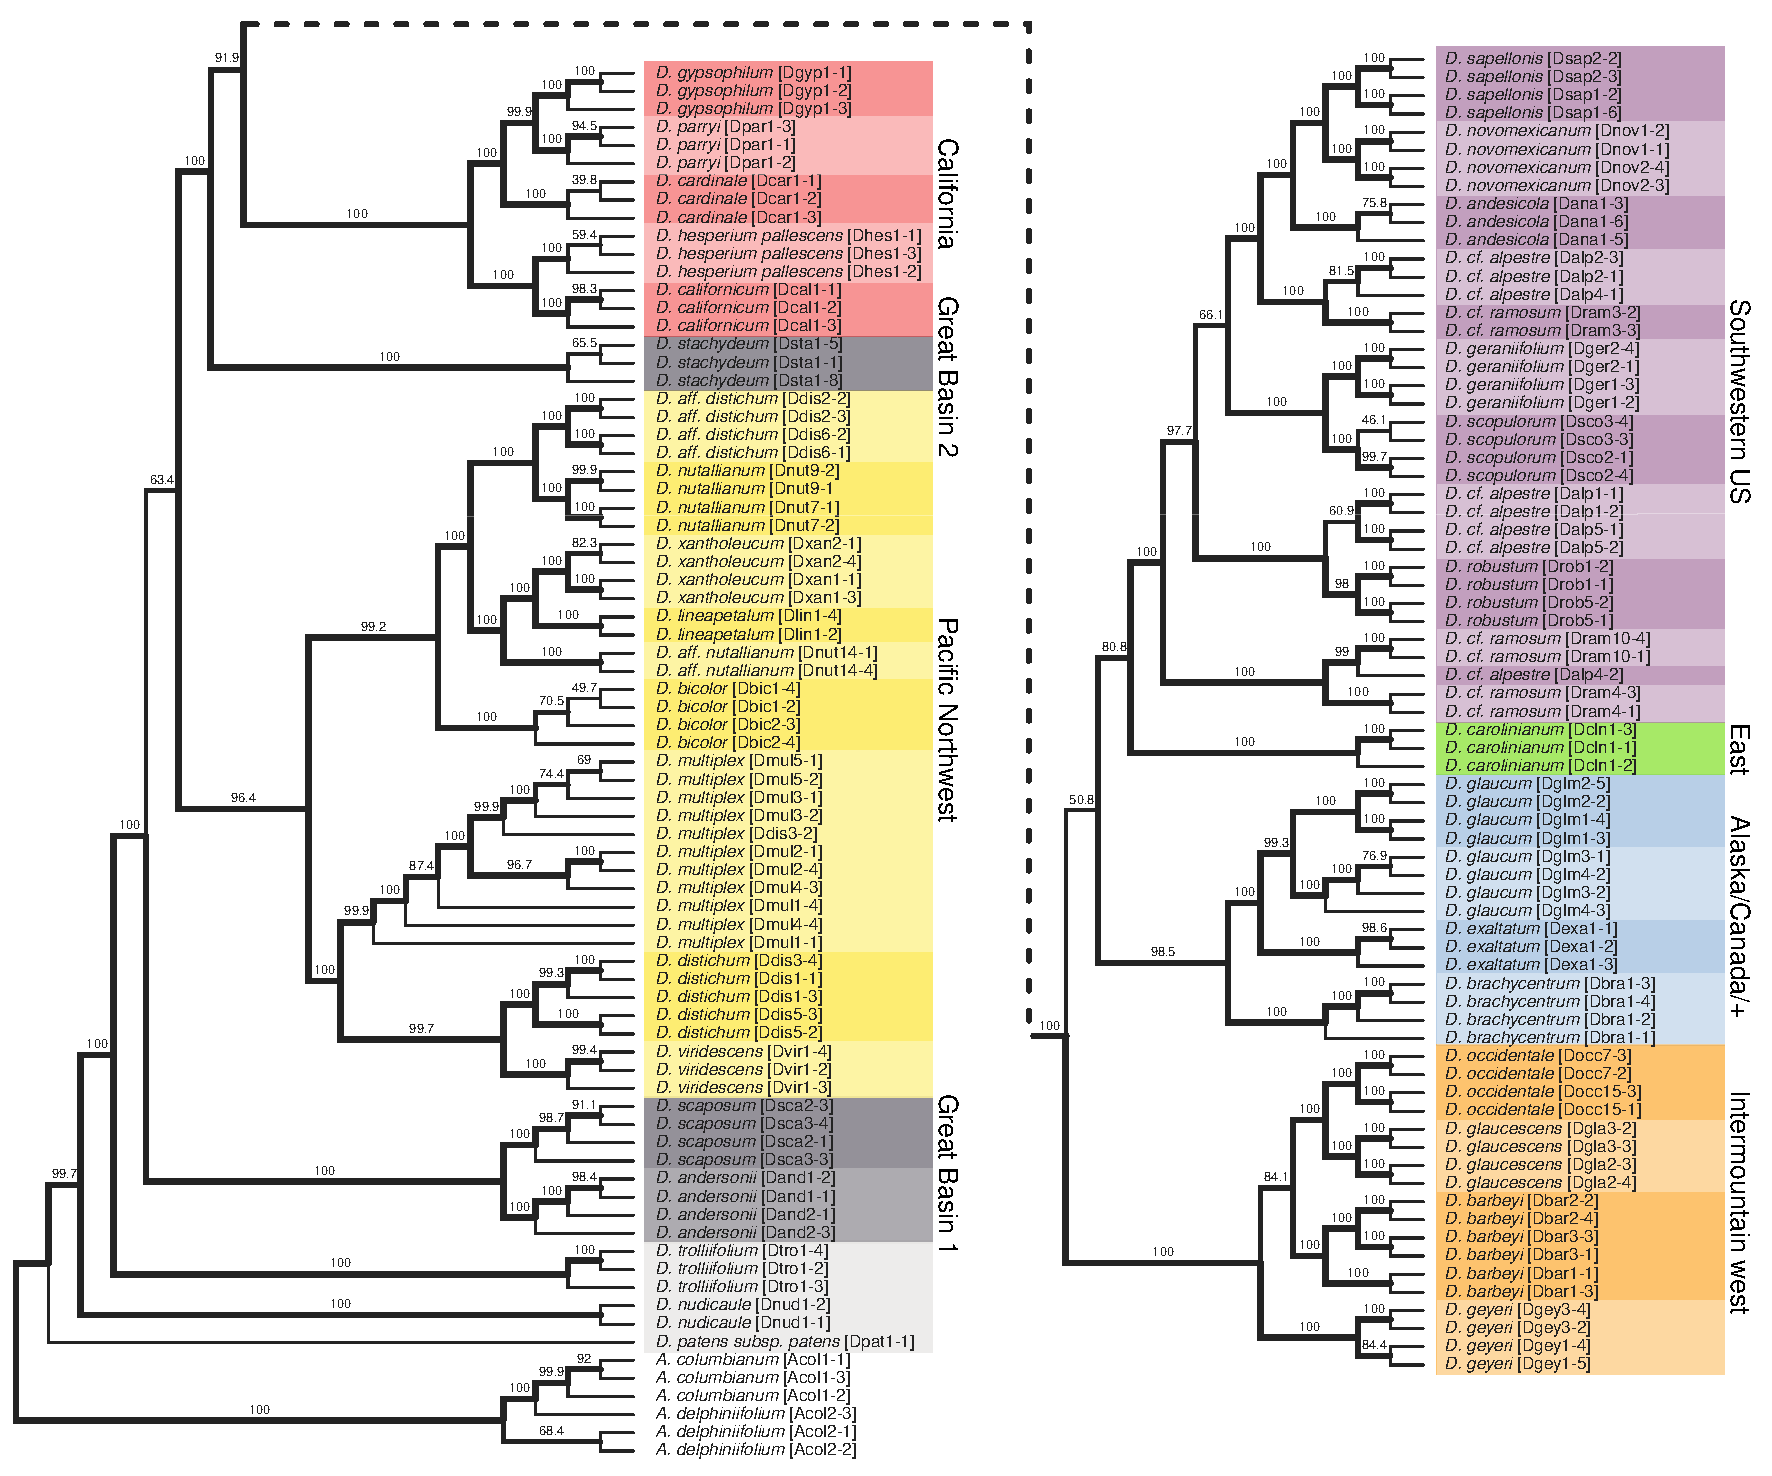
\includegraphics[width=0.99\textwidth]{./figures/caster-trees.pdf}	
	\caption{
		A rooted phylogenetic tree for 150 samples of \emph{Delphinium} sect. \emph{Diedropetala}
		inferred from the min10 SNP dataset using caster-site. Colored rectangles highlight
		groups that correspond well with discrete geographic regions, representing higher-level 
		clades. Replicate samples within each taxon form monophyletic clades, except in the case
		of \emph{D. distichum}, \emph{D. nuttallianum}, \emph{D. ramosum}, and \emph{D. alpestre}.
	}
	\label{fig:bigtree}
\end{figure}


\subsection{Principal component analysis}
We used principal components analysis (PCA) to further investigate patterns of
population structure and admixture among species and populations. Because PCA 
analyses are sensitive to missing data, we applied filtering and imputation 
using the \emph{ipyrad-analysis} toolkit PCA tool, which is specifically 
designed to address missing data common to RAD-seq datasets. 
% 
We ran three PC analyses, one for each hybrid-complex described above. 
In each analysis, we assigned samples to groups based on evidence from 
both their geographic sampling locations and their grouping into clades 
during phylogenetic analyses. These groups were used during imputation to 
probabilistically assign missing genotype calls based on allele frequencies
within each group. 
In \emph{ipyrad} this corresponds to the ‘sample’ imputation
method, with the ‘minmap` and ‘mincov` parameters set to 0.5, to only retain 
and call missing SNPs at sites where at least 50\% of the samples from all 
populations had data present. 
To reduce the effect of linkage, each analysis was run for 25 replicates
that subsampled a single SNP per RAD locus, and PCA visualizations show 
the variation across replicate runs and the centroid point for each sample.



%%%%%%%%%%%%%%%%%%%%%%%%%%%%%%%%%%%%%%%%%%%%%%%%%%%%%%%%%%%%%%%%%%%%%%%%%%%%%%
%%%%%%%%%%%%%%%%%%%%%%%%%%%%%%%%%%%%%%%%%%%%%%%%%%%%%%%%%%%%%%%%%%%%%%%%%%%%%%
%%%%%%%%%%%%%%%%%%%%%%%%%%%%%%%%%%%%%%%%%%%%%%%%%%%%%%%%%%%%%%%%%%%%%%%%%%%%%%
%%%%%%%%%%%%%%%%%%%%%%%%%%%%%%%%%%%%%%%%%%%%%%%%%%%%%%%%%%%%%%%%%%%%%%%%%%%%%%
%%%%%%%%%%%%%%%%%%%%%%%%%%%%%%%%%%%%%%%%%%%%%%%%%%%%%%%%%%%%%%%%%%%%%%%%%%%%%%
\section{Results}
\subsection{Genomic ddRAD sequencing and assembly}
Genomic sequencing yielded a mean of 1,071,118 (+/- S.D. 712,371) raw reads 
across all samples, which were assembled into relatively similar numbers of 
\emph{de novo} clusters within each sample (mean +/- S.D = 19,261 +/- 7,331). 
% 
We dropped samples with fewer than 1000 clusters. 
After clustering across the remaining samples and applying filters, 
the `min4' dataset included 80,169 loci, with the total alignment size of
150 samples x 6,490,732 sites (85.93\% missing) and contained 556,493 
SNPs (68.80\% missing). 
The `min10' dataset included 29,196 loci with a total alignment size of 
150 samples x 2,652,279 sites (70.96\% missing) and contained 399,001 SNPs
(58.03\% missing).


\subsection{Phylogenetic inference recovers monophyletic clades}
All phylogenetic analyses recovered similar topologies, with individuals of the same 
taxonomic determination consistently grouped into monophyletic clades. Few exceptions
were observed within \emph{D. ramosum}, \emph{D. alpestre}, \emph{D. distichum}, and 
\emph{D. nutallianum}, which we address later in the context of admixture.
% 
Caster-site recovered the same tree topology from both the `min4' and `min10' 
datasets (Fig.~\ref{fig:bigtree}, Fig.~\ref{fig:S1}), while the ML trees
inferred by raxml-ng differed from each other, and from the caster topology.
% 
These differences are concentrated on the backbone of the tree in the order 
of higher-level relationships that generally have low support across all trees 
(Fig.~\ref{fig:S2},~\ref{fig:S3}).
% 
Tree distances, measured using the generalized Robinson-Foulds mutual clustering
information metric \citep[MCI;][]{smith_information_2020}, show that the two
ML topologies share 93.3\% of information in common, while the caster topology
shares 86.0 and 91.3\% of information in common with the ML min4 and min10 
trees, respectively.


A set of higher level clades was recovered across all trees that shows a strong
concordance with biogeographic regions.
This includes taxa associated with Great Basin, Pacific Northwest, California, 
Intermountain West, Alaska/Canada, the Southwestern US, and Eastern North America
(Fig.~\ref{fig:sptree}a-b). 
% 
All of our tree hypotheses support three early diverging lineages that split
from the rest of our sampled \emph{Delphinium} taxa early in the radiation. 
This includes \emph{D. patens}, \emph{D. nudicaule}, and \emph{trollifolium},
which are distributed in central California, northern California, and northern 
California and the Pacific Northweest, respectively. We focus most of our further
analyses and discussion on the larger recovered clades in our study.
% 


\begin{figure}[t!]
	\centering
	\includegraphics[width=0.95\textwidth]{./figures/Fig2_sptree.pdf}
	\caption{
		Phylogeny and biogeographic distribution of \emph{Delphinium} sect. \emph{Diedropetala}.
		(a) Sampling locations of \emph{Delphinium} used in this study.
		Color codes correspond to distinct biogeographic regions associated with phylogenetic clades
		(yellow: Pacific Northwest,
		 red: California,
		 orange: Intermountain west,
		 blue: Alaska and Canada,
		 green: Eastern USA,			
		 purple: Southwestern USA,
		 black: Great Basin,
		 grey: other)
		(b) A rooted species tree topology inferred from the min10 SNP dataset using caster-site with 
		population mapping of 150 individuals to 41 populations, shown with local block bootstrap supports.
		% 
		One or more biogeographic states occupied by each taxon are shown in a colored marker next to each tip.
		%
		Our results conflict with the current taxonomic treatment in the Flora of North America (Warnock 1997)
		derived from morphology, as indicated by subsection designations next to each taxon name.
		% 
		(c-f) There is substantial conflict across the backbone of the tree, and different methods or
		datasets recovered different topologies. 
		Support for monophyly of each clade was consistently >95\%, as indicated by values at the tips
		of each tree. Support for internal nodes generally showed greatest conflict with respect to the
		placement of the ALCA and PNW clades.
		(g) Representative images of \emph{Delphinium} sect. \emph{Diedropetala} 
		(Photo credits: \emph{D. viridescens} from the Burke Herbarium, 
		and \emph{D. xantholeucum} from Eastern Washington University).
	}
	\label{fig:sptree}
\end{figure}


Support for the monophyly of each higher-level clade is >95\% in all trees, 
but they conflict in the order of relationships among these clades and the 
support for these splits (Fig.~\ref{fig:sptree}c-f).
% 
A grouping of clades IMW, ALCA, ENA, and SW is recovered with 100\% support
across all trees, but their order of relationships within this clade also 
varies among trees.
% 
The BAS1 and PNW clades tend to be recovered near the base of the tree, while
the placement of the CAL clade is more variable and tends to have low support.
This may be a result of admixture between species in the CAL clade and other
early diverged lineages that also occur in California, which we examine below.
% 
Given the uncertainty in the order of relationships among these higher-level 
clades, and our incomplete taxon sampling, it would be premature to draw strong
conclusions from our results about the order and dynamics of historical biogeography
in this clade.
% 
Nevertheless, our finding of strongly supported clades that correspond to distinct
biogeographic regions represents a major revision to our understanding of the 
phylogeny of \emph{Delphinium} sect. Diedropetala, suggesting need for a major 
taxonomic revision.
% 
% In the following sections, we focus on elucidating the impact of hybrid admixture 
% on our phylogenetic hypotheses.



\subsection{Higher-level clades correspond strongly with biogeographic regions}

We designate eight named clades that were consistently recovered across our
phylogenetic analyses and correspond well to geographic regions. None of our
clades correspond uniquely with an existing taxonomic subsection in Warnock's
FNA treatment (Fig.~\ref{fig:sptree}b). 

% Consistent clades.
The BAS1 clade occurs in the Great Basin and includes \emph{D. scaposum} and
\emph{D. andersonii}. 
% While these taxa are currently placed in the subsection
% Subscaposa, other members of this subsection are spread across several clades of 
% the phylogeny.
Our sampled populations of \emph{D. scaposum} are from SE Nevada and NW Arizona, 
and the populations of \emph{D. andersonii} from southern Idaho. 
% 
The BAS1 clade does not group with the other taxon we sampled from the Great
Basin, \emph{D. stachydeum}, from northern Nevada. This taxon occurs as the 
sole member of its clade, which we designate BAS2.

The PNW clade corresponds to taxa distributed in mountainous regions of the Columbia 
plateau in E Washington, NE Oregon, Idaho, and W Montana. It includes \emph{D. lineapetalum}, 
\emph{D. xantholeucum}, \emph{D. nuttallianum}, \emph{D. distichum}, \emph{D. bicolor}, 
\emph{D. viridescens}, and \emph{D. multiplex}. We recover both \emph{D. nuttallianum}
and \emph{D. distichum} as polyphyletic, possiby as a result of admixture, which we
investigate further below. These five taxa are derived from four
different subsections in the Warnock taxonmic treatment. These seven taxa grouped
together in our results are derived from six different subsections in the current 
FNA treatment.

The CAL clade includes taxa distributed primarily in California, including 
\emph{D. californicum}, \emph{D. hesperium}, \emph{D. cardinale}, 
\emph{D. gypsophilum}, and \emph{D. parryi}. These five taxa grouped together in
our results are derived from four different subsections in the current FNA treatment.

The IMW clade corresponds to taxa distributed in the "intermountain west" region 
between the northern and souther Rocky Mountains.
It is represented by four species in our study, 
\emph{D. geyeri}, \emph{D. barbeyi}, \emph{D. occidentale}, and \emph{D. glaucescens}.
Several of these species have large geographic ranges spanning this region.

The ALCA clade corresponds to several widespread species that occur in Alaska
and Canada, and sometimes also elsewhere. This includes the widespread species
\emph{D. glaucum}, which we sampled in both Alaska and the Sierra Nevada; 
\emph{D. brachycentrum}, which we sampled in Alaska, but also extends into Asia;
and \emph{D. exaltatum}, which occurs broadly in eastern North America, but which 
we sampled Colorado near Boulder. The two populations of \emph{D. glaucum} group
monophyletically in the caster topologies, but \emph{D. glaucum} from Alaska groups 
with the \emph{D. brachycentrum} in the ML topologies.
% Members of this are all in the Exaltata subsection,
% representing the "tall larkspurs". 

The SW clade is represented by 10 taxa in our study which share a biogeographical
distribution throughout the southwestern United States. This includes 
\emph{D. scopulorum}, \emph{D. geraniifolium}, \emph{D. alpestre},
\emph{D. robustum}, \emph{D. ramosum}, \emph{D. andesicola}, \emph{D. sapellonis},
and \emph{D. novomexicanum}. 
% Notably, this clade includes many species 
% classified in subsection Exaltata, ibut our results show clearly that many species
% from Exaltata fall outside of this clade. Our 

%%%%%%%%%%%%%%%%%%%%%%%%%%%%%%%%%%%%%%%%%%%%%%%%%%%%%%%%%%%%%%%%%%%%%%%%%%%%%%%%%%%%%%%%
%%%%%%%%%%%%%%%%%%%%%%%%%%%%%%%%%%%%%%%%%%%%%%%%%%%%%%%%%%%%%%%%%%%%%%%%%%%%%%%%%%%%%%%%
%%%%%%%%%%%%%%%%%%%%%%%%%%%%%%%%%%%%%%%%%%%%%%%%%%%%%%%%%%%%%%%%%%%%%%%%%%%%%%%%%%%%%%%%

\subsection{Hybridization and Introgression}
Many \emph{Delphinium} species overlap both in geography and phenology in western 
North America, increasing their potential to hybridize. Results from the Fbranch
analysis show substantial admixture across the tree, both among close relatives as
well as among more distantly related taxa.
% 


% We focused our genomic tests for introgression on species that are resolved as 
% polyphyletic in one or more of our phylogenetic analyses, specifically complexes
% involving \emph{D. distichum}, \emph{D. multiplex}, and \emph{D. nuttallianum}; 
% \emph{D. brachycentrum} and \emph{D. glaucum}; 
% or \emph{D. ramosum}, \emph{D. robustum}, and \emph{D. alpestre}. 
% % 
% In each of these cases, one or few samples fell outside of the major clade that 
% included all other populations of that species in our phylogenetic analyses, 
% providing initial evidence for hybridization as a source of discordance. 
% In several cases, these polyphyletic signals are consistent with observations of 
% putative hybrids in Warnock’s FNA treatment, to which we refer readers for a more
% comprehensive description of hypothesized hybridization events in \emph{Delphinium}. 
% In the following sections, we describe the first genomic evidence applied to 
% investigate three specific introgression hypotheses.



\begin{figure}[t]
	\centering
	%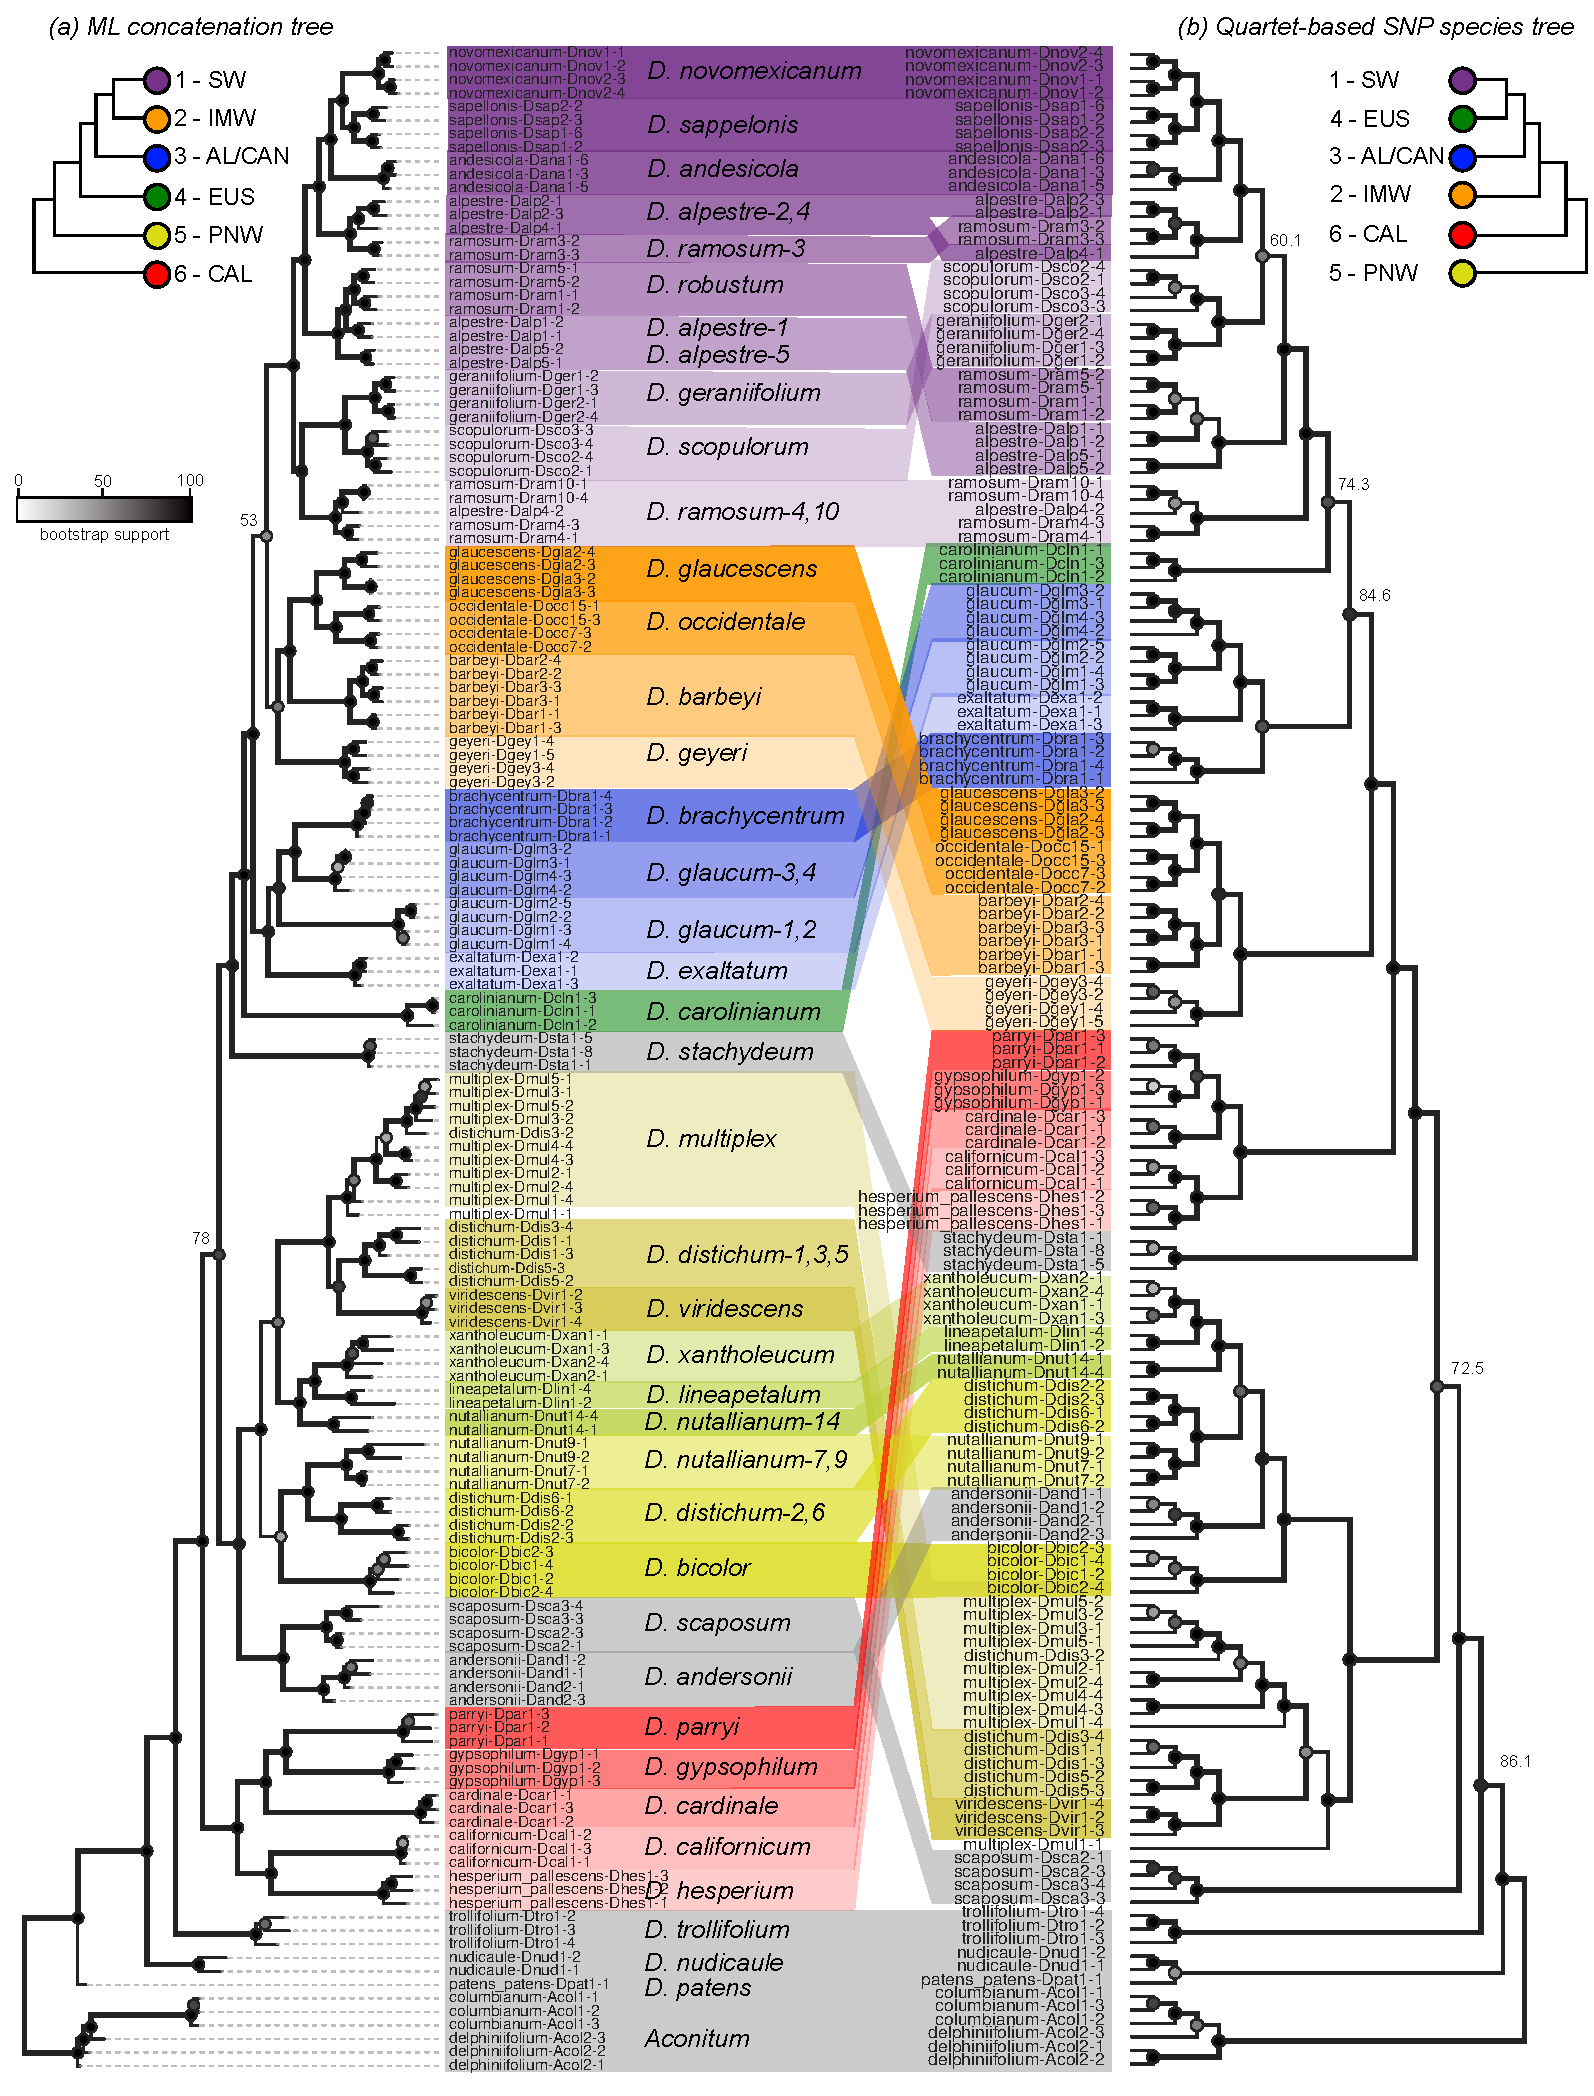
\includegraphics[width=0.99\textwidth]{./figures/trees_v2.pdf}
	\caption{
        Fbranch statistic ...
	}
	\label{fig:fbranch}
\end{figure}


\subsection{Hybrid complexes}

\subsubsection{D. andersonii}
Jepson says that \emph{D. andersonii} hybridizes with D. parishii and D. nuttallianum,
the latter of which is included in our sampling. Our tests for admixture confirm
that hybridization between these taxa has led to introgression.
in NE California, SE Oregon, central Idaho, or southern Utah. 


\subsubsection{D. nuttallianum}
A widespread species complex that is both geographically and elevationally widespread (300--3300 m) and 
described as an extremely difficult species complex. 
Note: Hybridizes with Delphinium andersonii, Delphinium depauperatum, Delphinium nudicaule, Delphinium polycladon; extremely difficult, variable complex.


\subsubsection{D. nudicaule}
Red flowered species is generally hummingbird pollinated and distributed in Coastal and N California and S Oregon. It is hypothesized to hybridize with D andersonii, D antoninum, D decorum, D depauperatum, D luteum, D. nuttallianum, D. patens, and D. trolliifolium. 


We next tested for evidence of genomic admixture consistent with stated evidence
of observed hybrids in nature. In Warnock's FNA treatment \emph{D. barbeyi} is 
described as hybridizing extensively with several species, including 
\emph{D. ramosum} and \emph{D. sapellonis} from clade 1, and with 
\emph{D. glaucum} from clade 3, of which the hybrid intermediates have been 
classified as \emph{D. occidentale}, a taxon we have many samples of, and
which consistently groups into clade 1 (separate from the two clades 2 and 3, 
where its putative progenitor species are grouped). 


Delphinium barbeyi hybridizes extensively with D. glaucum in western Colorado and eastern Utah, where plants appearing to be hybrid [ D . × occidentale (S. Watson) S. Watson] are often far more common than plants of either putative parent. Several other names have been used for these plants, including D . elatum var. occidentale S. Watson, D . abietorum Tidestrom, and D . scopulorum subsp. occidentale (S. Watson) Abrams. Delphinium barbeyi is also known to hybridize with D . ramosum and D . sapellonis .


\subsection{Admixture in clade 4 and \emph{D. distichum complex}}
Taxonomists have hypothesized that \emph{Delphinium distichum} hybridizes with both 
\emph{D. multiplex} and \emph{D. nuttallianum} 
(referred to as \emph{D.} x \emph{diversicolor} Rydberg; Warnock, 1997).
% 
The morphological differences among these three taxa are subtle, forming a complex that 
is difficult to untangle. 
% 
In our phylogenetic analyses, both \emph{D. distichum} and \emph{D. nuttalianum} were
resolved as paraphyletic (Fig.~\ref{fig:2}). Because their history of hybridization
may involve additional closely related species, we examined signatures of admixture
among all seven species in clade 4. 
% 

\begin{figure}[t!]
	\centering
	  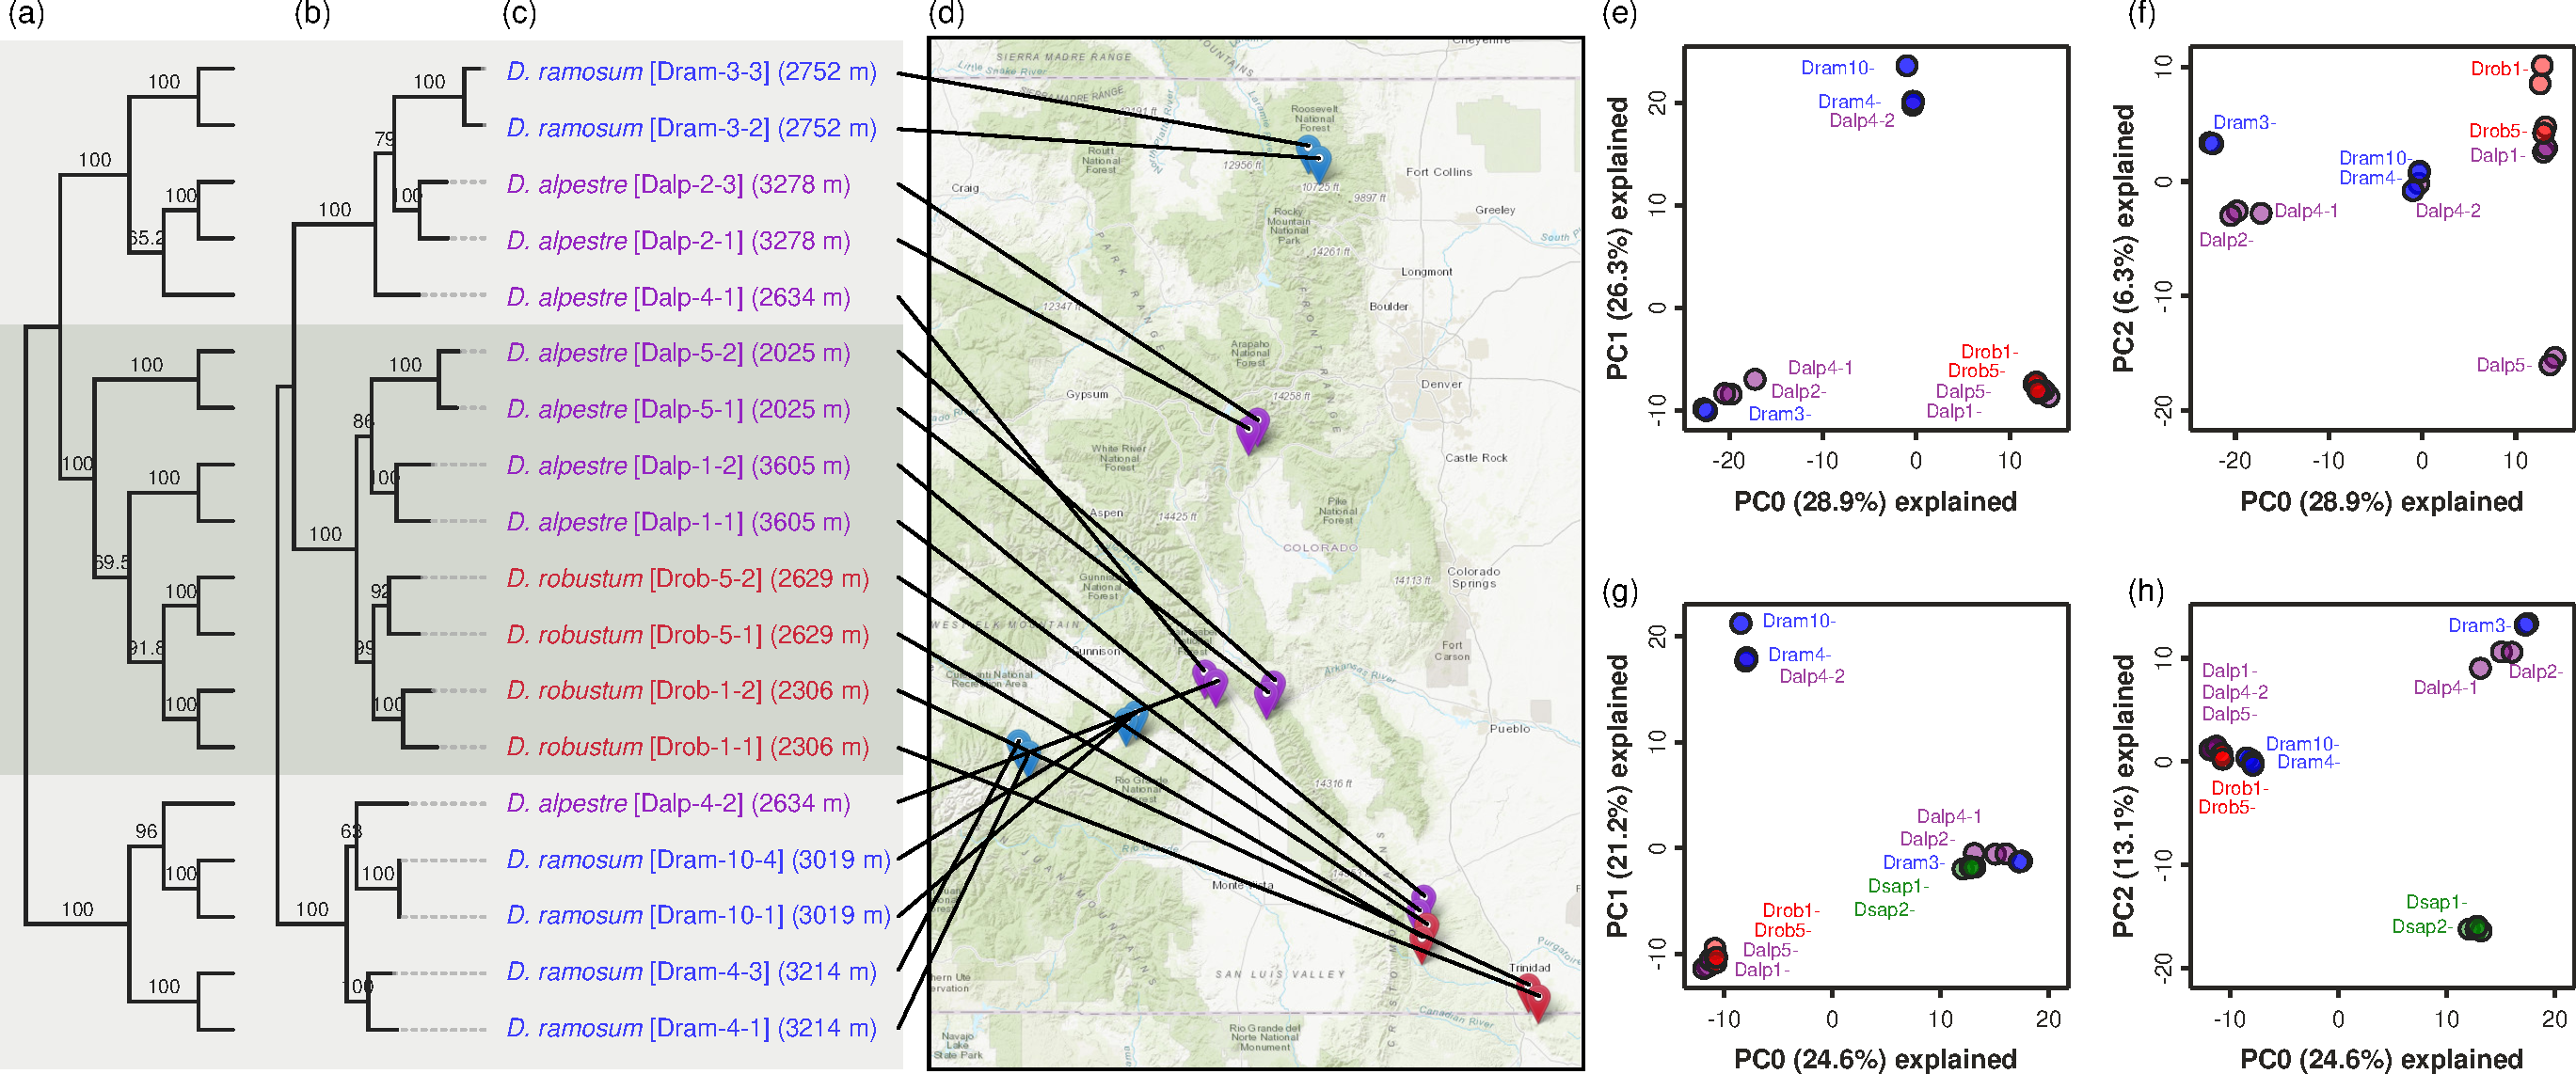
\includegraphics[width=0.99\textwidth]{./figures/ramosum-robustum-alpestre2}	
	\caption{
        Hybrid complex of \emph{D. robustum}, \emph{D. ramosum}, and \emph{D. cf. alpestre} in the Southern Rocky Mountains. 
        (a-b) Three distinct clades are consistently supported in our phylogenetic analyses, which corresponding more closely with geography than with species determinations based on morphology.
        (c-d) Phylogenetic analyses focused on the subset of samples in this complex
        recovers the same three clades, with similar topologies recovered by caster-site and raxml-ng, respectively.
        (e-f) PCA of the subset of samples in this hybrid complex.
        (g-h) PCA with the inclusion of \emph{D. sapellonis}, which shows evidence of admixture.        
	}
	\label{fig:robustum}
\end{figure}


% PCA analysis.


% BABA
Using our phylogenetic hypotheses that identified geographically distinct clades corresponding
to these taxon names, we tested for evidence of genomic introgression using D-statistics. 
All of our phylogenetic analyses supported two separate 
\emph{D. distichum} clades, the first (\emph{D. distichum}-1,3,5) groups with 
\emph{D. viridescens} and \emph{D. multiplex}, while the other 
(\emph{D. distichum}-2,6) groups with \emph{D. nutallianum}-7,9. 
Geographically, populations 2 and 6 of \emph{D. distichum} are on the border of 
Washington and Idaho nearby populations of \emph{D. nuttallianum}, whereas 
populations 1, 3, and 5 are in central Washington nearby populations of 
\emph{D. multiplex} and \emph{D. viridescens}. 


To resolve this issue, we first tested whether the two clades comprising populations assigned the name D. distichum are in fact two distinct lineages or a result of admixture with other species. We analyzed ABBA-BABA statistics for hypotheses that compared D. distichum-1,3,5 as an introgressive donor to test whether it shared greater relatedness with D. distichum-2,6 relative to that taxon’s closer relatives on the tree, D. nuttallianum-7,9 and D. bicolor (tests 0-1; Fig. 3; Table S2). Neither of these tests were significant at a threshold of alpha=0.05 (Z=2.73, ABBA=212.85, BABA=174.95 for test with D. nuttallianum-7,9; Z=2.71, ABBA=232.02, BABA=188.58 for test with D. bicolor). We also tested the reverse direction, with D. distichum-2,6 as an introgressive donor into D. distichum-1,3,5 relative to its closest relatives, D. multiplex or D. viridescens (tests 2-3; Fig. 3; Table S2). These tests were also non-significant (Z=1.64, ABBA=192.54, BABA=171.14 for test with D. multiplex; Z=1.16, ABBA=139.92, BABA=125.55 for test with D. viridescens). These results suggest that the two distinct clades that were morphologically determined as D. distichum are in fact two distinctly derived lineages that do not share extra ancestry with each other as would be expected if one or both species was a product of hybrid introgression.


We ran a number of additional tests to examine potential admixture involving other species in this complex. The most significant D-statistics show admixture between D. nuttallianum-7,9 and  a clade of three taxa including \emph{D. nuttallianum-14} (Fig. 3; tests 15, 18, 21, 29, 32, 35, 38, 41, and 44). This could explain the polyphyletic splitting of D. nuttallianum, where populations 7, 9, and population 14 show evidence of admixtureis in fact an admixed population. Whereas the two distinct clades of D. distichum show no evidence of admixture, and may represent cryptic speciation, the two distinct clades of D. nutallianum do appear admixed, suggesting this taxon may represent a hybrid morphotype, at least at the sampling locations examined here. For now, we included D. nutallianum-7,9 and D. distichum-1,3,5 as representatives of these taxa in our species-level tree, but further investigation of their taxonomic distinctiveness is needed.
% For this reason we consider D. nuttallianum-7,9 as the correct placement for D. nuttallianum. Based on the 100\% bootstrap support between D. distichum-2,6 and D. nuttallianum-7,9 in our RAxML phylogeny (Fig. S1), we considered D. distichum-1,3,5 as the correct placement of D. distichum in the clade with D. viridescens and D. multiplex.


%%%%%%%%%%%%%%%%%%%%%%%%%%%%%%%%%%%%%%%%%%%%%%%%%%%%%%%%%%%%%%%%%%%%%%%%%%%%%%%%% 
%%%%%%%%%%%%%%%%%%%%%%%%%%%%%%%%%%%%%%%%%%%%%%%%%%%%%%%%%%%%%%%%%%%%%%%%%%%%%%%%% 
%%%%%%%%%%%%%%%%%%%%%%%%%%%%%%%%%%%%%%%%%%%%%%%%%%%%%%%%%%%%%%%%%%%%%%%%%%%%%%%%% 
\subsection{Admixture in clade 3 and the \emph{Delphinium glaucum} complex} 
Despite substantial morphological differences between D. brachycentrum and D. glaucum, Warnock’s FNA treatment mentions that hybrids between these two species have been referred to as Delphinium x nutans A. Nelson. Based on our ABBA-BABA tests, D. brachycentrum and D. glaucum-3,4 from Alaska show evidencesigns of admixtureintrogression with D. occidentale (Fig. 4, Table S3; tests 2-3, 16-17, 20-21). This makes sense geographically, since sSamples identified as D. x nutans have been found at the northern edge of D. occidentale’s range and southern edge of D. brachycentrum’s range in British Columbia, where D. glaucum is abundant [CITE]., so introgression between these three species is certainly plausible. By contrast, D. exaltatum, a species endemic to eastern North America, provides a standard against which to examine the amount of introgression between these two clades. Tests 5, 10, 19, 23, and 27 show that D. exaltatum shows a lack of admixture with the subclade that includes D. occidentale, compared to its relatives D. glaucum and D. brachycentrum, which are more strongly admixed with D. occidentale. In fact, tests 28-31, suggest that D. glaucum-3,4 and D. branchycentrum each share sequentially less ancestry with D. exaltatum, respectively, likely as a result of their increased amounts of introgression from D. occidentale. 
% 
% Additionally, although D. glaucum-3,4 and D. brachycentrum appear as closer relatives than D. glaucum-1,2 in our ML tree, the ABBA-BABA test involving these three taxa shows D. glaucum-1,2 as more similar to D. glaucum-3,4 than D. brachycentrum (Fig. 4, Table S3; test 28), indicating that our D. brachycentrum samples truly are hybrids. Interestingly, D. exaltatum from the eastern U.S. appears to have experienced introgression with D. glaucum-1,2 and D. glaucum-3,4 (Fig. 4, Table S3; tests 29-30) indicating that populations of 
D. glaucum is widespread, its range spanning the North American Cordillera from Alaska down through California and Colorado, where it may have the potential to hybridize with additional different species according to geographic proximity. These patterns of introgression and population structure need to be investigated further with more samples and populations of D. glaucum, D. brachycentrum, and D. exaltatum. Based on these results, we dropped D. brachycentrum from our final species tree and represented D. glaucum as a single tip.


\begin{figure}[t]
	\centering
	%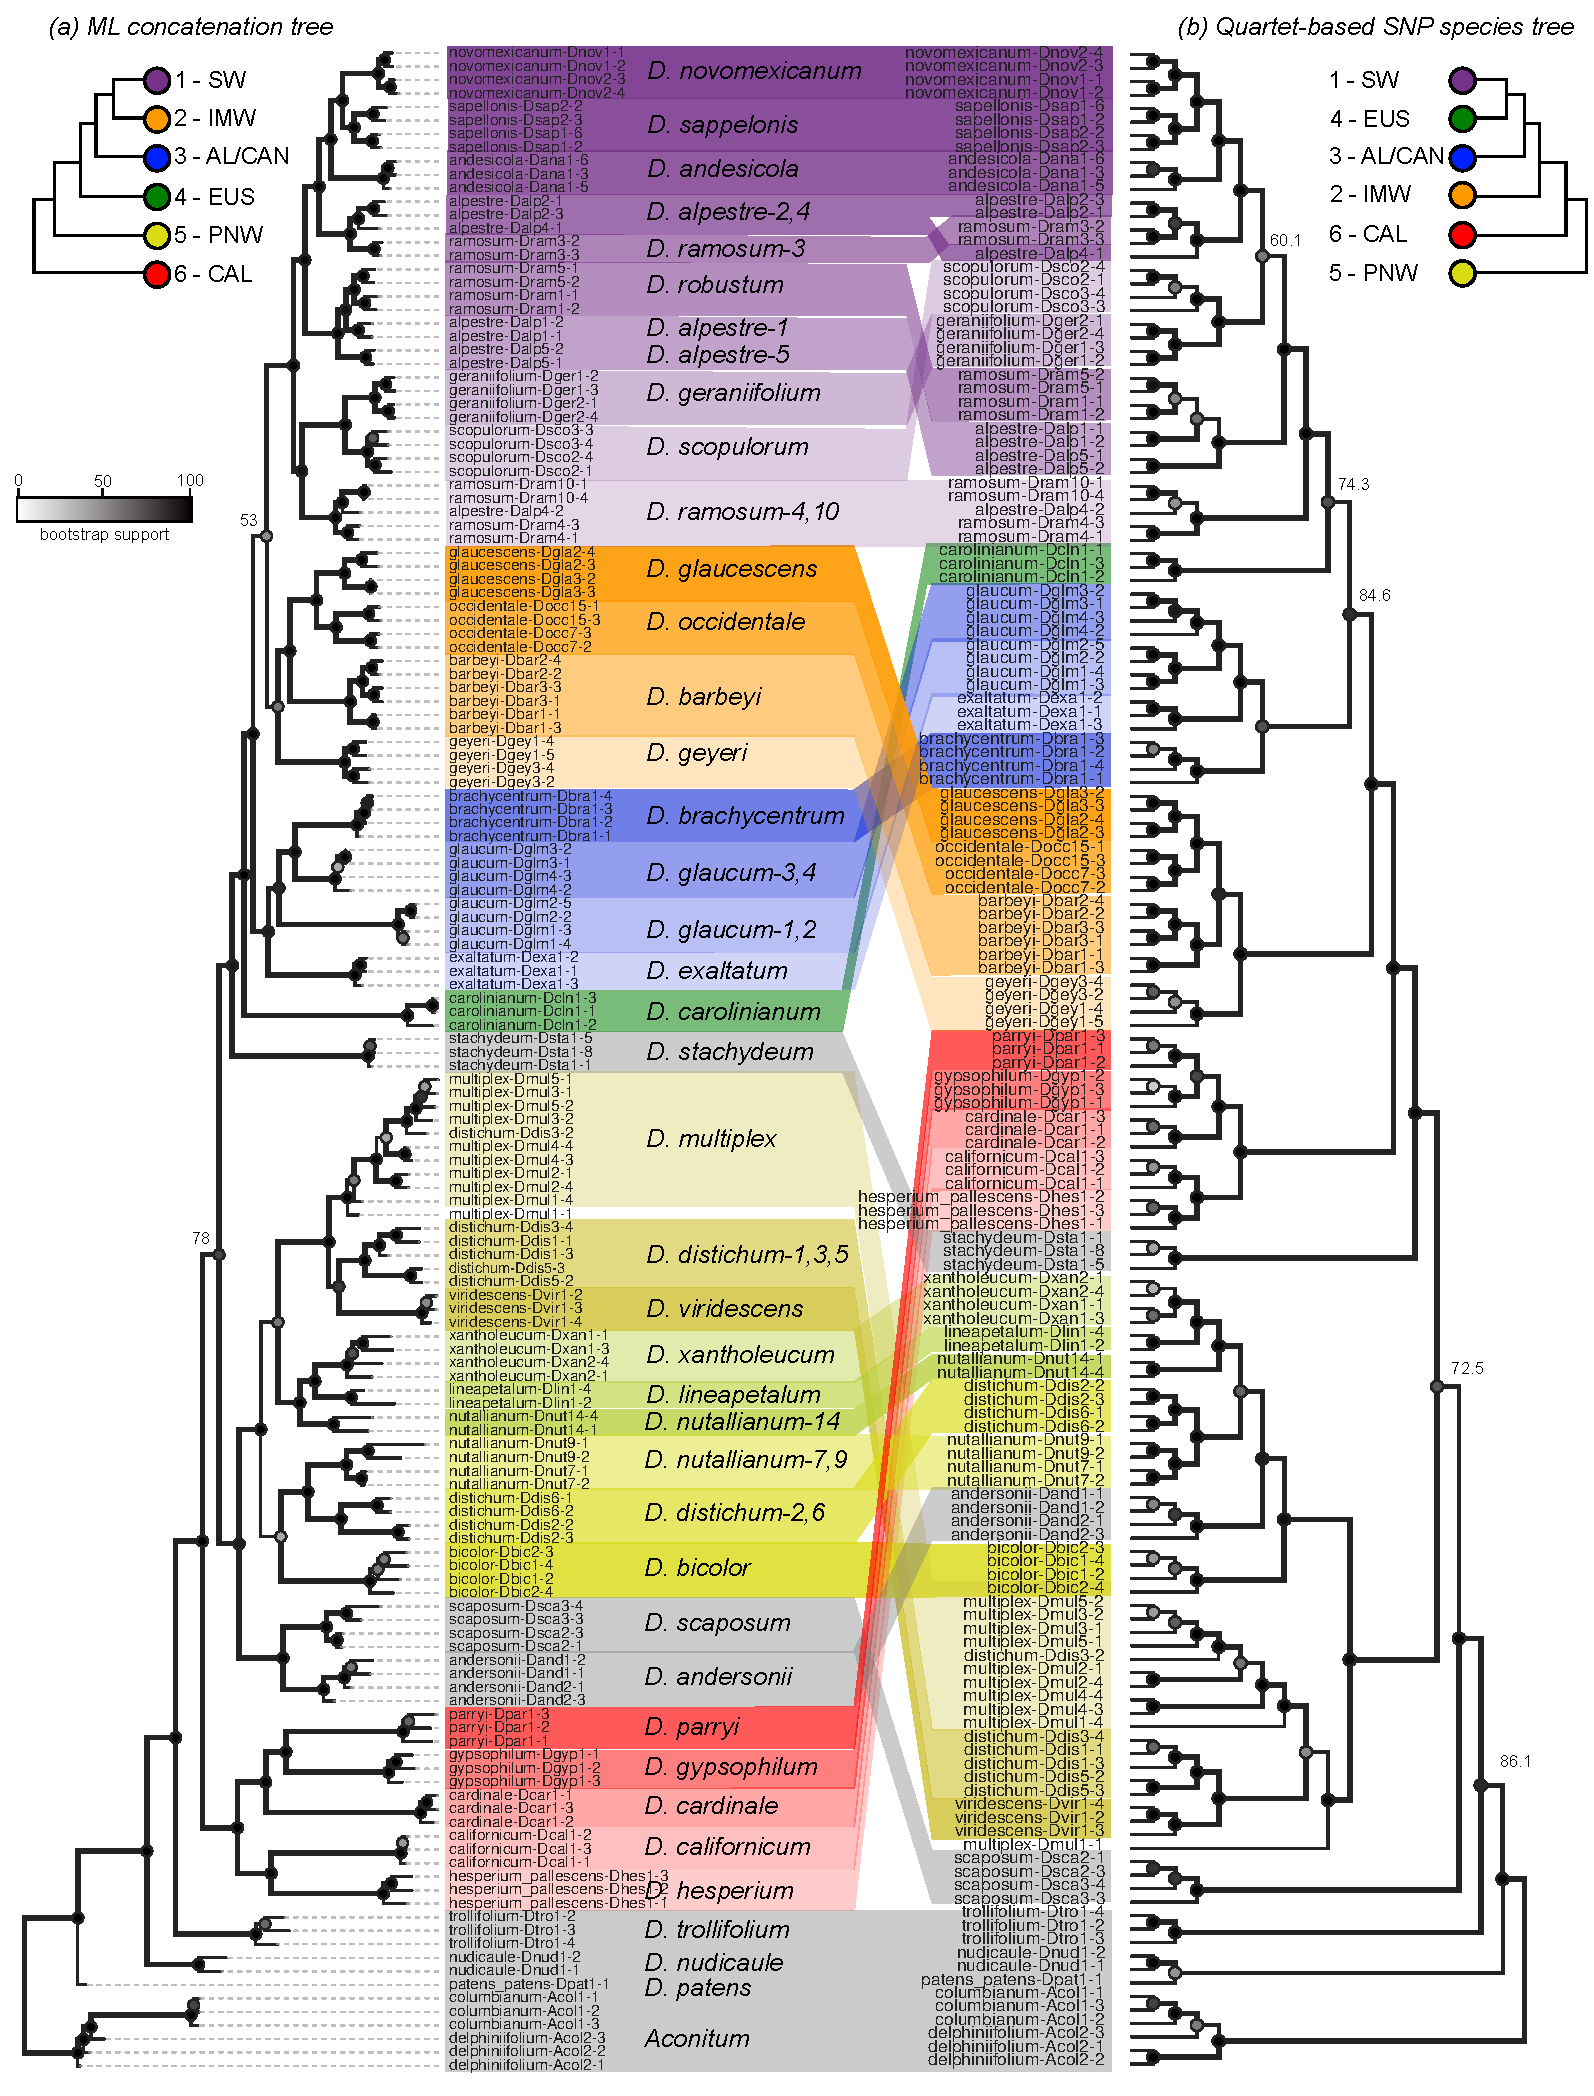
\includegraphics[width=0.99\textwidth]{./figures/trees_v2.pdf}
	\caption{
        Zoom into map + PCA of glaucum complex.
	}
	\label{fig:5}
\end{figure}



\subsection{Admixture in the \emph{Delphinium ramosum} complex}
There is substantial disagreement across floras concerning the distinction between Delphinium ramosum, D. robustum, and D. alpestre (Ewan 1945, Warnock 1997, Weber 2012, Ackerfield 2015), a complex of species native to Colorado and New Mexico. Our dataset includes multiple populations of each species. We conducted ABBA-BABA tests between these populations and the other five species that form a clade located geographically in the southwestern U.S. Based on these tests, prevalent introgression among these taxa is causing polyphyletic signals in our tree that are unresolvable with our current dataset (Fig. 5, Table S4). Notably, taxa that came out polyphyletic on the tree, such as D. ramosum and D. alpestre, do not show significantly greater amounts of admixture than other taxa in this clade. We left the polyphyletic taxa from this clade unresolved in the final species tree.


\begin{figure}[t]
	\centering
	%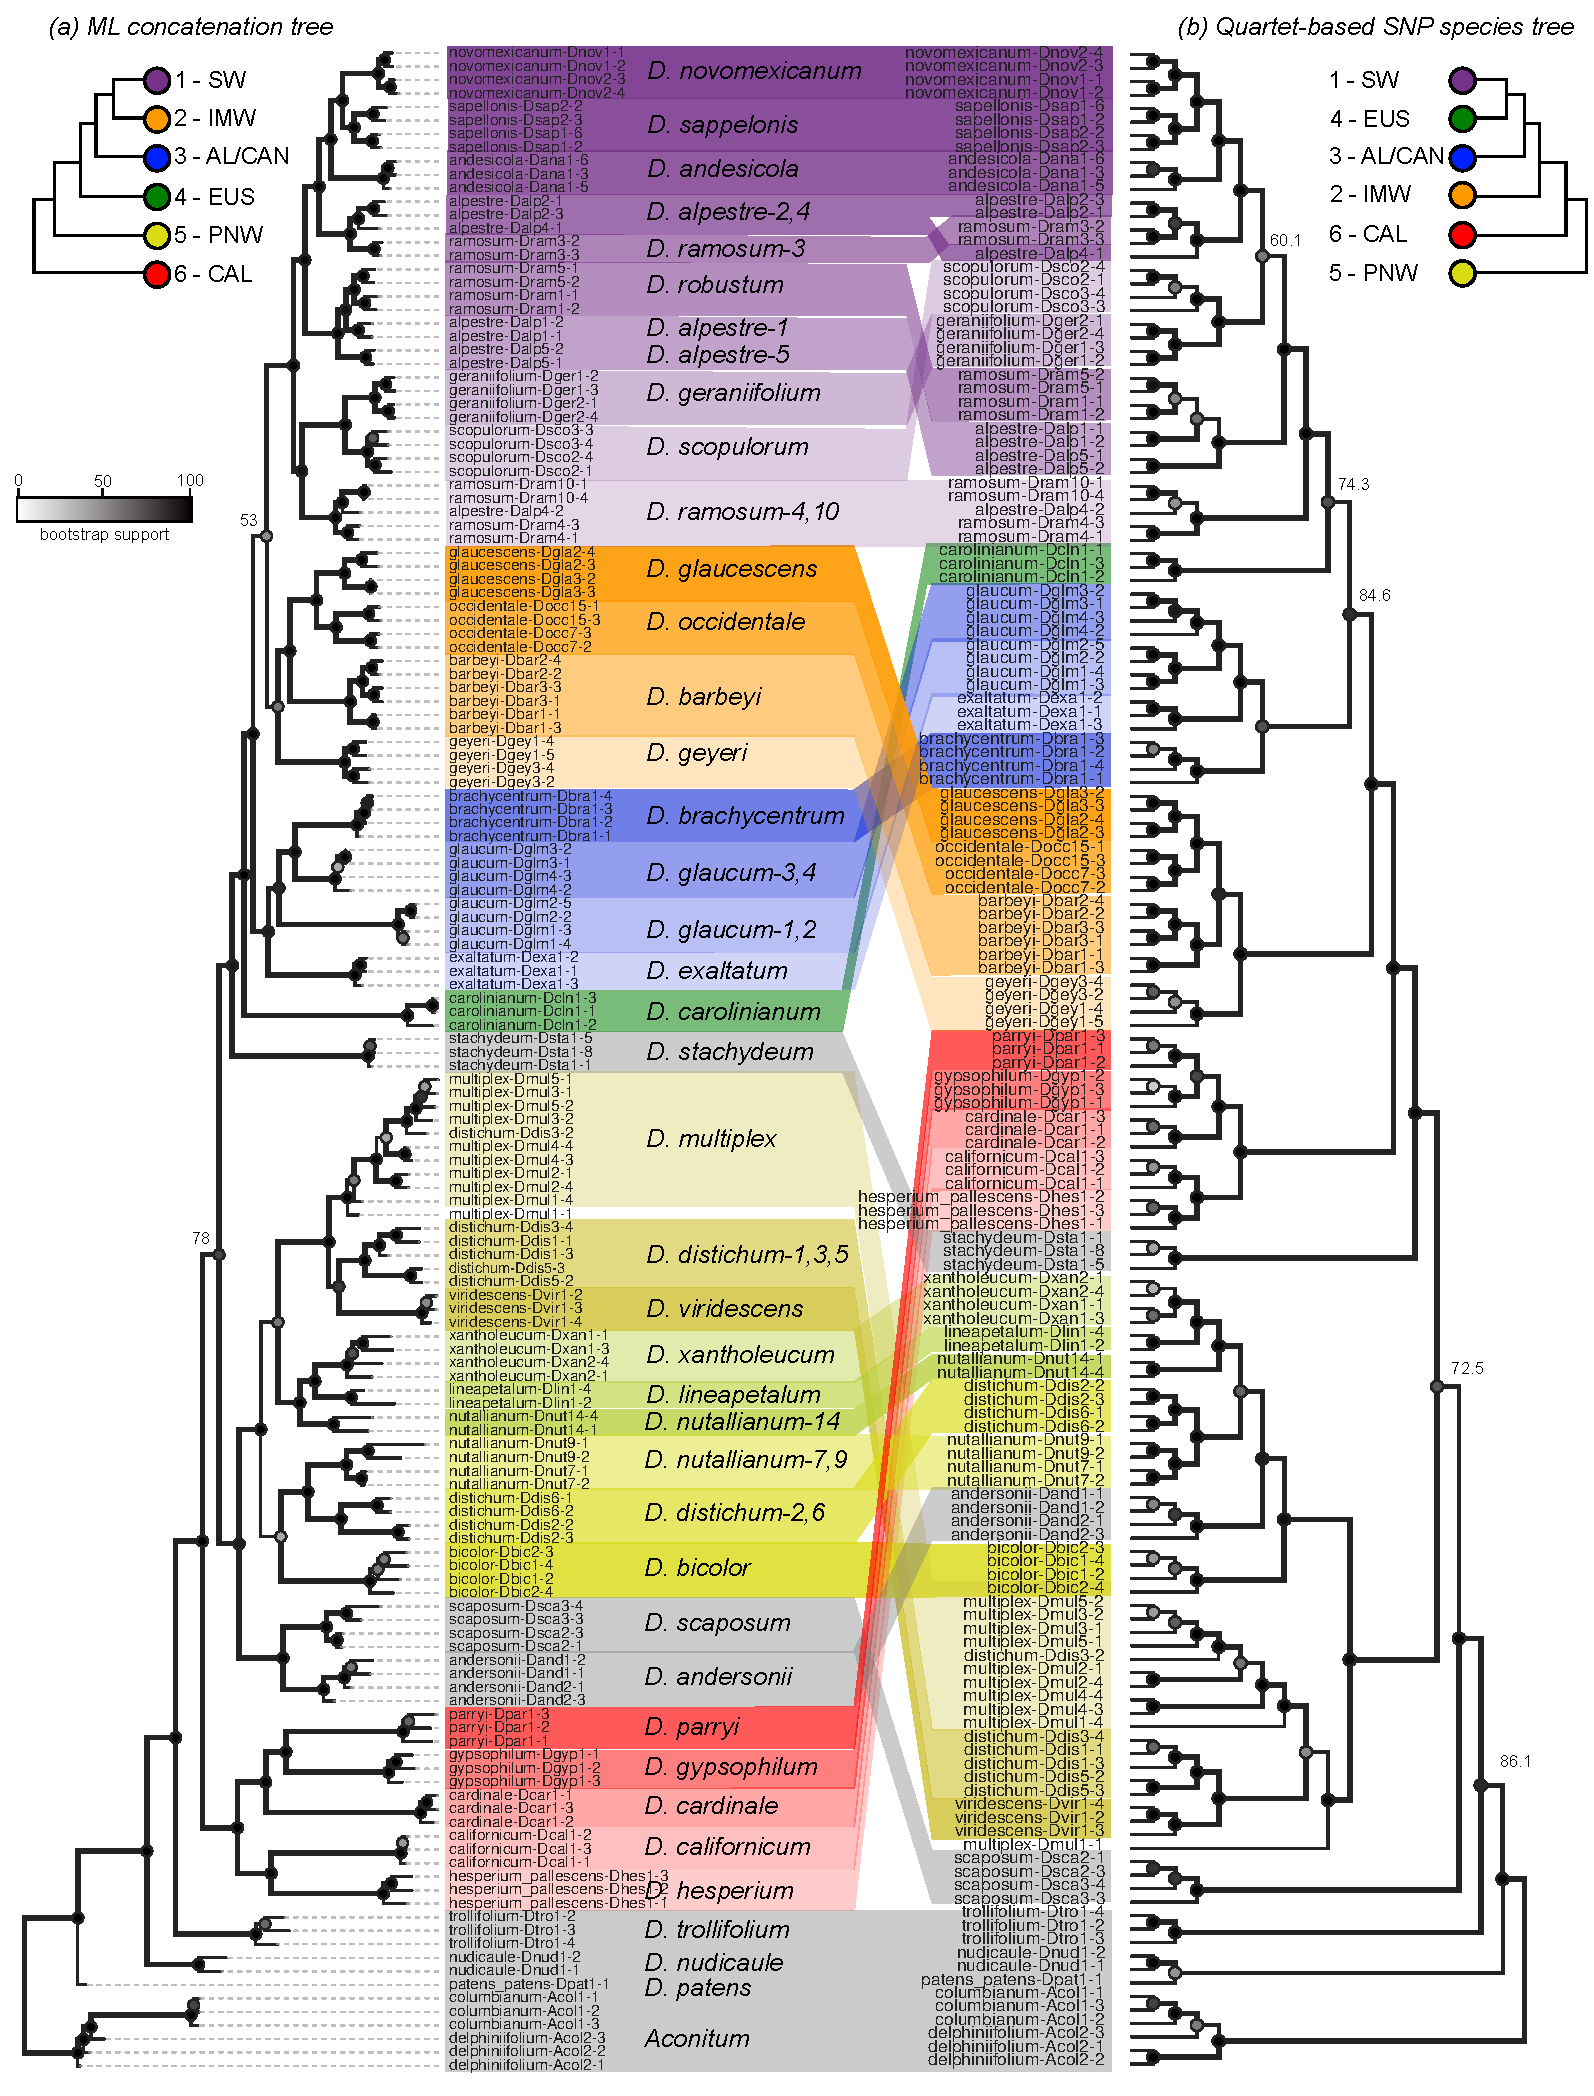
\includegraphics[width=0.99\textwidth]{./figures/trees_v2.pdf}
	\caption{
        Zoom into map + PCA of ramosum complex.
	}
	\label{fig:6}
\end{figure}



\section{Discussion}

% summarize broad results
We generated a large-scale phylogenomic dataset to resolve phylogenetic relationships 
among populations and species spanning 34 taxa in the North American clade \emph{Delphinium}
sect. Diedropetala. Our results recovered most populations within species as monophyletic,
and grouped many species into a few monophyletic clades associated with biogeographic regions.
However, genomic admixture tests reveal abundant evidence of hybridization between species both
within and between clades. 

% how does this relate to broad existing classifications
This is consistent with previous taxonomic work that split the clade into sixty species 
on the basis of distinct morphological variation, including leaf, flower, and root variation.
However, while we do not have a complete taxon sampling of the \emph{Delphinium} sect. 
Diedropetala clade, the relationships in our species tree topology are highly conflicting 
with most subsection groupings proposed by Warnock in the Flora of North America (Fig. 1).
Indeed, eight of the nine subsections were recovered as polyphyletic in our tree, 
highlighting the need for an updated taxonomic treatment for this group in light of
molecular evidence.

% 
The ‘min4’ RAxML phylogeny had strong support across most backbone nodes, but the 
three most difficult clades to resolve involved species belonging to the 
\emph{D. distichum}, \emph{D. glaucum}, and \emph{D. ramosum} complexes. 
Despite this lack of resolution, we ultimately decided on the final species phylogeny
after testing for introgression and conducting PCA analyses for each of these complexes.
While we are confident in the majority of relationships across the final phylogeny,
these complexes need to be further verified with increased genomic sampling and
morphological analysis.



Among the clades described in Warnock or FNA none was fully supported by our 
phylogenomic analyses. Previous section names were generally quite discordant
with our results. The 

 sampled eleven species from this
The Exaltata subsection of "tall larkspurs", as described by Warnock,
includes at least 14 species that typically grow at high elevation or 
latitude, and grow to large size. 
subsection

in North America 
brachycentrum
alpestre Rydb.
ramosum Rydb.
sapellonis
novomexicanum
occidentale (indicated as a hybrid)
exaltatum
andesicola
robustum (Northern New Mexico, southern Colorado)
ramosum
glaucescens
glaucum.


\emph{D. californicum} can be easily confused with \emph{D. glaucum} or \emph{D. exaltatum}, and
is most readily distinguished by its western distribution and earlier flowering time [CITE FNA]. 
It is, however, quite distantly related in our results.



Importantly, our collections and analyses will help resolve long-standing disagreements concerning the taxonomy of multiple species. For example, we included multiple samples of \emph{D. occidentale}, 
a species recognized by Ewan (1945) and Holmgren (2012), but which Warnock (1997) describes as
a hybrid between \emph{D. glaucum} and \emph{D. barbeyi}. 
Our replicate sampling tree (Fig. 2) and PCA analysis (Fig. 6B) shows that \emph{D. occidentale}
as distinct from these two species, and more closely related to \emph{D. glaucescens}
than either of them with 100\% bootstrap support.

Further exploration of D. occidentale’s population structure would prove useful in raising it back to species status. Additionally, our analysis of the Delphinium ramosum complex underscores the possibility that Delphinium alpestre is not a single taxon, but rather two separate taxa that independently speciated into alpine environments following the split of a progenitor population of Delphinium ramosum or robustum. Considering that these taxa belong to the most recently diverged clade of Delphinium sect. Diedropetala, future research involving these species may be a fruitful avenue for studies involving convergent plant adaptation in mountain environments.

The potential bias of missing data on phylogenetic inference should not be overlooked. To reduce this bias, we inferred multiple phylogenies using maximum-likelihood and multispecies-coalescent-based methods on datasets with varying amounts of missing data. Despite some disagreement between these methods, our final species-level phylogeny is a vast improvement over previous molecular phylogenies which relied on single-locus markers and failed to resolve relationships within this clade.

Add a couple sentences about tall larkspurs being longer-lived vs. shorter-lived perennials and how that trait maps onto the tree pretty well.
Biogeography hypothesis; asia - north america disjunctions; what else dispersed to NA at this time? Other plant genera that might support this hypothesis of glacial extirpation and then migration from south to north?

Overall, our phylogenomic analyses present new hypotheses and insights into the evolutionary history of this rapidly radiating clade, and demonstrate that the divergence history of this group is much more complex than morphology alone reveals. Future work should include the remaining unsampled taxa so that questions concerning biogeographic history, dispersal, and diversification linked to climatic, topographical, or pollination shifts (Sharma et al., 2024) since Delphinium’s arrival to North America can be tested. While a full sampling of all Delphinium sect. Diedropetala species is required, the need for a major revision of higher-level taxonomy within this clade is clear, which should aim to identify morphological characteristics among species that are concordant with the monophyletic clades supported by molecular evidence.


\bibliographystyle{ecol_let}
\bibliography{references}  



\beginsupplement

\begin{figure}[p]
	\centering
	% \includegraphics[width=0.95\textwidth]{./figures/Fig2_sptree.pdf}
	\caption{
		A rooted phylogenetic tree for 150 samples of \emph{Delphinium} sect. \emph{Diedropetala}
		inferred from the min4 SNP dataset using caster-site, with supports shown from
		1000 local block bootstrap replicates. 
		Colored rectangles highlight
		groups that correspond well with discrete geographic regions, representing higher-level 
		clades. Replicate samples within each taxon form monophyletic clades, except in the case
		of \emph{D. distichum}, \emph{D. nuttallianum}, \emph{D. rasomum}, and \emph{D. alpestre}.
	}
	\label{fig:S1}
\end{figure}

\begin{figure}[p]
	\centering
	% \includegraphics[width=0.95\textwidth]{./figures/Fig2_sptree.pdf}
	\caption{
		A rooted phylogenetic tree for 150 samples of \emph{Delphinium} sect. \emph{Diedropetala}
		inferred from the min4 sequence alignment using raxml-ng, with supports shown from
		200 non-parametric bootstrap replicates. 
		Colored rectangles highlight
		groups that correspond well with discrete geographic regions, representing higher-level 
		clades. Replicate samples within each taxon form monophyletic clades, except in the case
		of \emph{D. distichum}, \emph{D. nuttallianum}, \emph{D. rasomum}, and \emph{D. alpestre}.
	}
	\label{fig:S2}
\end{figure}

\begin{figure}[p]
	\centering
	% \includegraphics[width=0.95\textwidth]{./figures/Fig2_sptree.pdf}
	\caption{
		A rooted phylogenetic tree for 150 samples of \emph{Delphinium} sect. \emph{Diedropetala}
		inferred from the min10 sequence alignment using raxml-ng, with supports shown from
		200 non-parametric bootstrap replicates. 
		Colored rectangles highlight
		groups that correspond well with discrete geographic regions, representing higher-level 
		clades. Replicate samples within each taxon form monophyletic clades, except in the case
		of \emph{D. distichum}, \emph{D. nuttallianum}, \emph{D. rasomum}, and \emph{D. alpestre}.
	}
	\label{fig:S3}
\end{figure}



\end{document}



